% !TEX root = ../TechProject.tex

\graphicspath{{Chapter5/}}


\chapter{Application}

Inspired by the training of a fader estimation paper \citep{kim_automatic_2017}, mixesdb.com is a website of archived DJ sets. With other 260,000 mixes on the site, using this as a dataset to train my model proved to be an excellent choice. As mentioned in Chapter 2, Daniel Chow built a system that takes in a single song and outputs similar songs based on the mixesdb dataset \citep{chow_music_2020}. His code will provide the foundation as I implement multiple inputs and add an extra layer of validation.

For simplicity sake, I won't use any deep learning implementation.

\subsection{Data set}
As Chow details, data was srcaped from the website MixesDB done using Selenium. The tracks in a given DJ Set which had a corresponding Spotify link were stored with a given user ID for the DJ.  In cases where a single DJ set included multiple DJs, the set was considered as belonging to all the DJs involved, and the corresponding songs were linked to each DJ's user ID. The data was then organised in such a way that

\begin{figure}[H]
	\hspace*{-1.8cm}   
	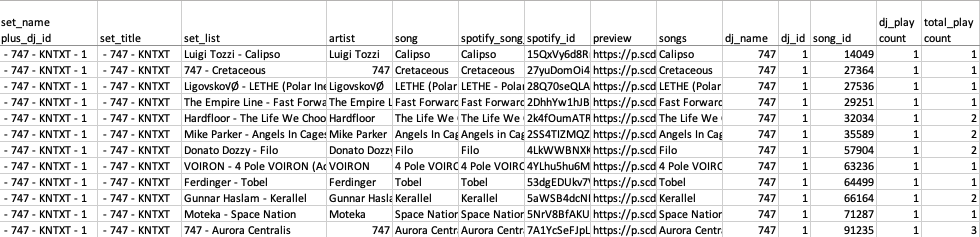
\includegraphics[scale=0.55]{images/dataset}
	\centering
	\caption{Table showing a DJ Set in the dataset} 
\end{figure}

Figure 5.1 shows a DJ Set entry in the dataset. Each song has a link to a preview due to the spotify id being accessible.


\subsection{Initial Suggestions}
The inital suggestions part of the model is made using Alternating Least Squares, a matrix factorisation algorithm that was made popular by the Netflix Prize award. As explained in chapter 2, this is both an affectively computational way of handling a dataset, and splitting up a matrix to its latent factors reveals trends in between songs and DJs.

A model is made from the dataset, then a list of songs gets inputted. A for loop is ran that will find similar items with the ALS algoritm for each song. the number of recommended song suggestions for each song was set to 200, to assure a large amount of similar songs are used in the next part of the model.

\begin{figure}[H]
	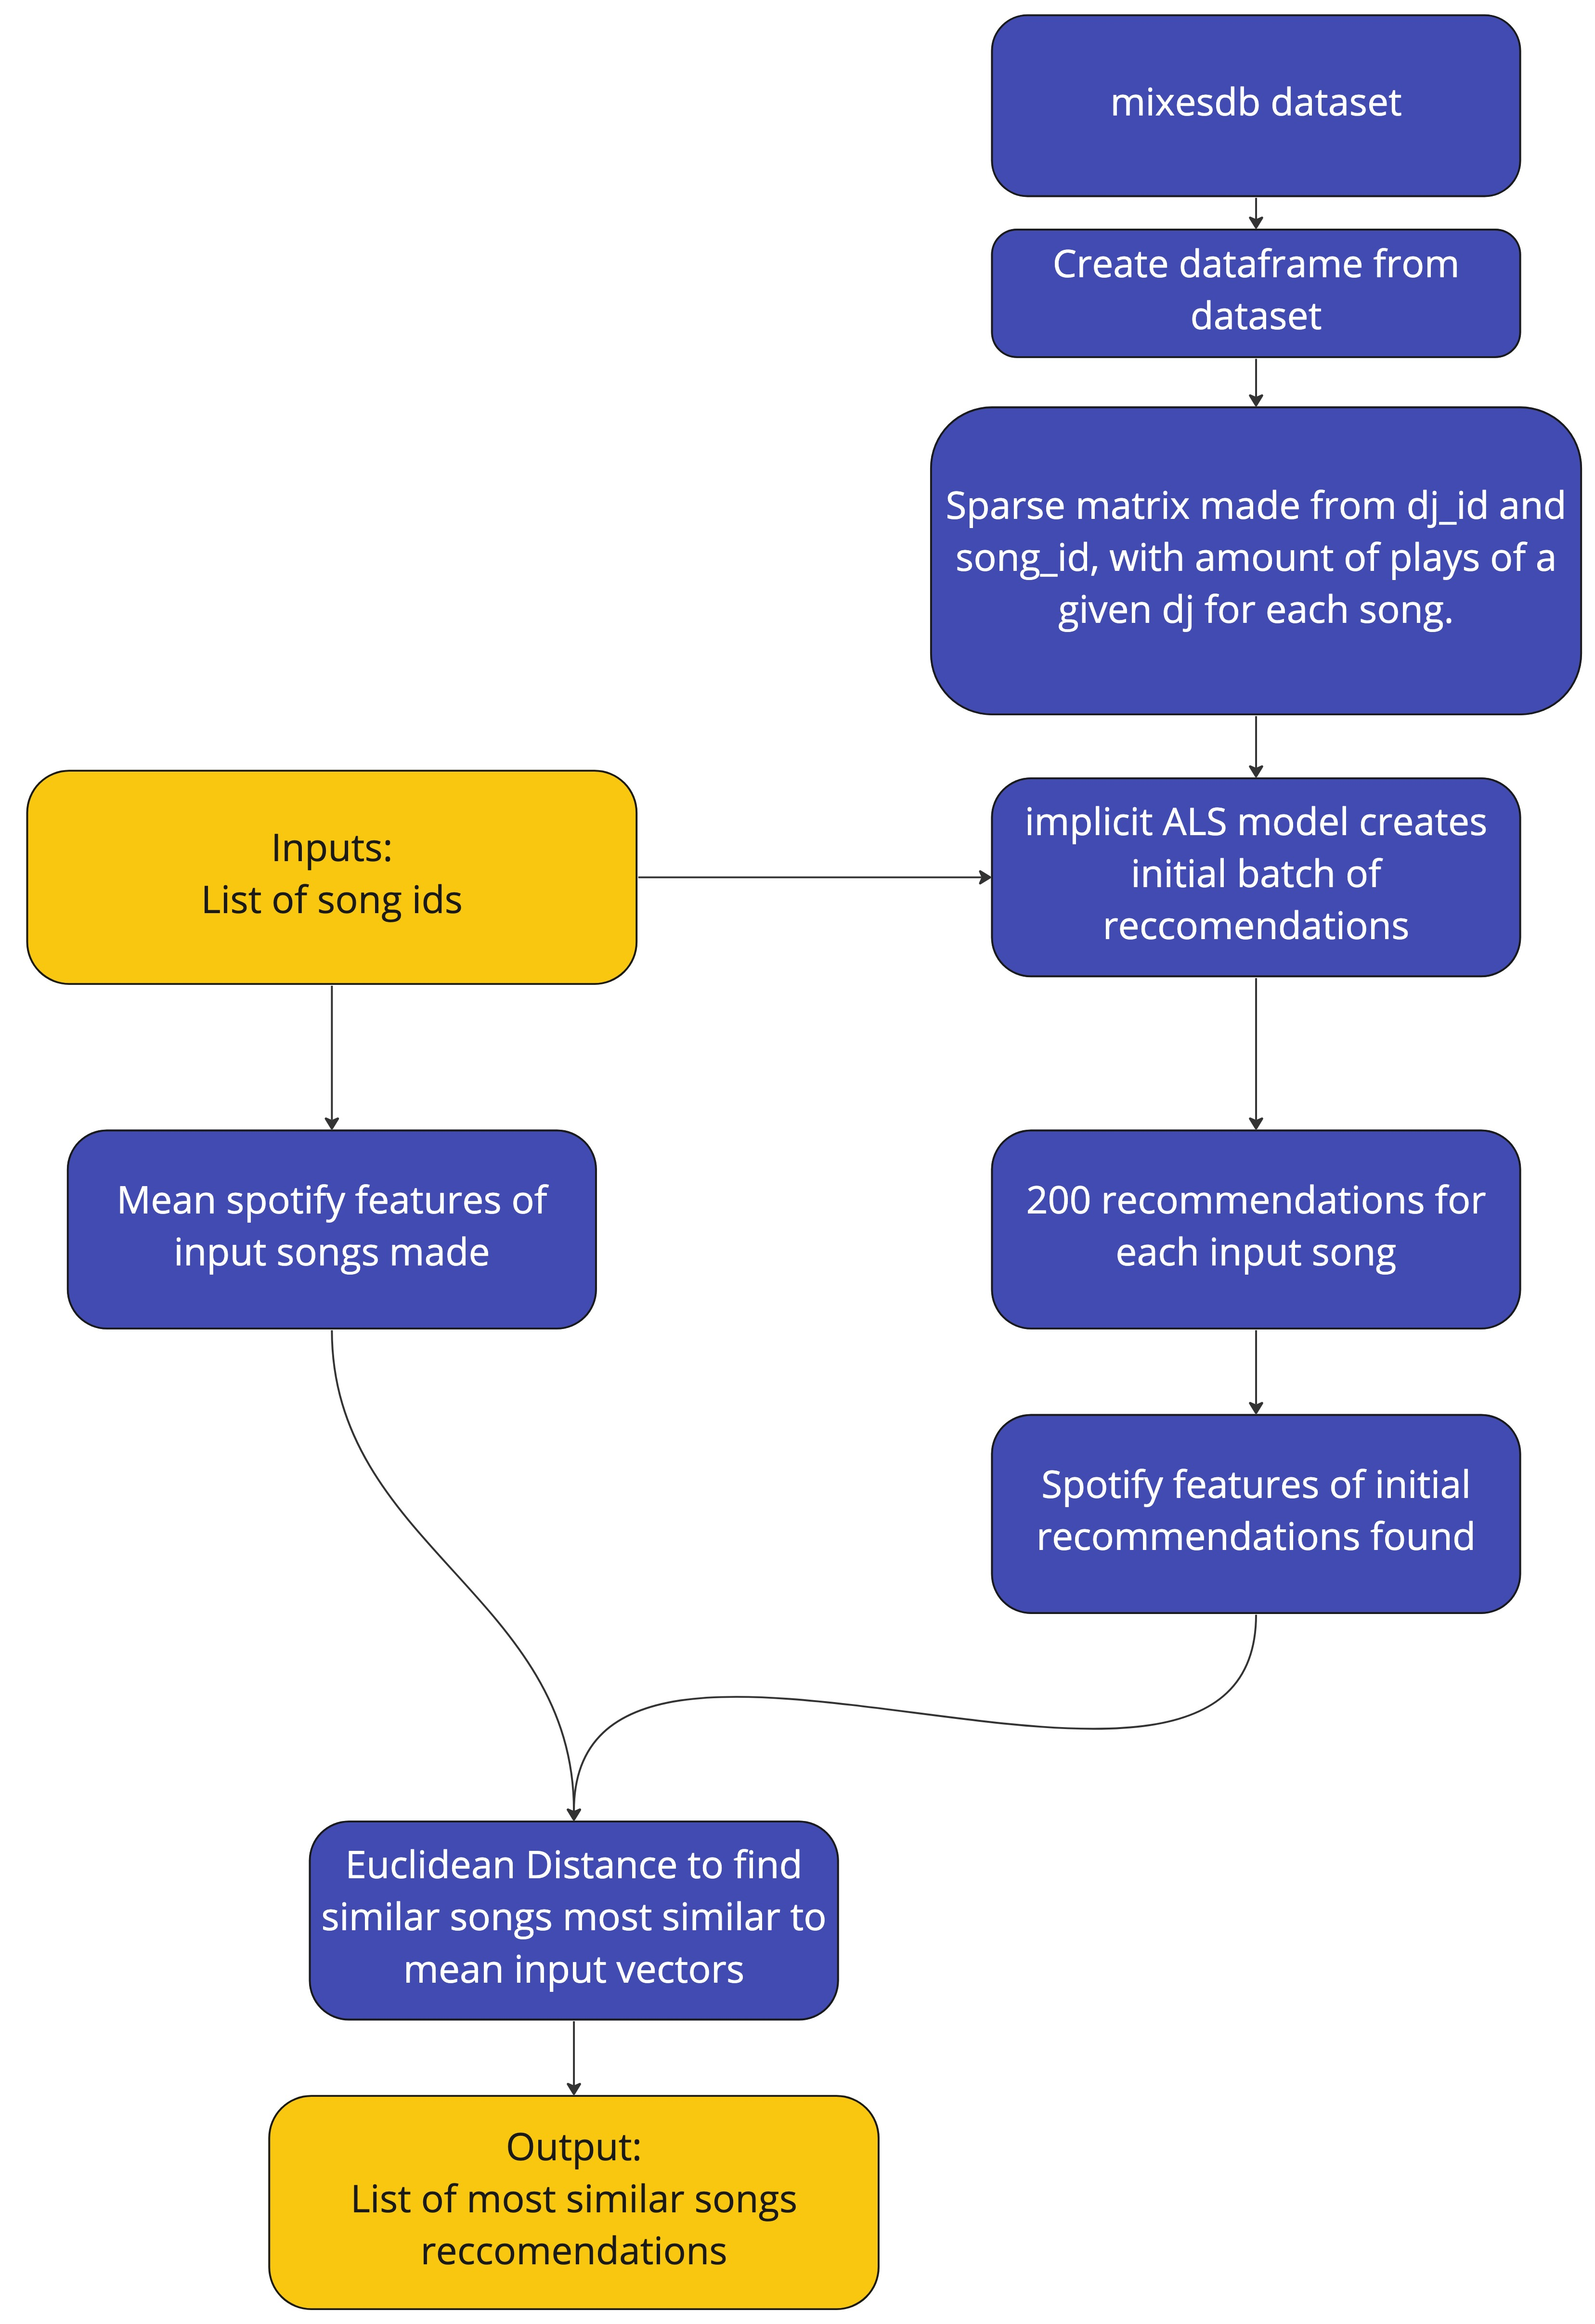
\includegraphics[scale=0.1]{images/application_app_flow}
	\centering
	\caption{Application flow of the application} 
\end{figure}

\subsection{Final Suggestions}
As of yet the code used is similar to Daniel Chows, aside from iterating through many song inputs, instead of one. To add an extra layer of filtering, the spotify API is used to further explore which songs are the most similar.

Using both the input songs, and initital suggestions, using the spotify ID a variety of audio features can be found. They are as listed:

\begin{enumerate}
	\item \textbf{acousticness} - A measure on how acoustic the song sounds (1 being definitely acoustic  )
	\item \textbf{danceability} - Measurement on how suitable a track is for dancing based on tempo, rhythmic features and overall regularity. 1.0 is most danceable. 
	\item \textbf{energy} - a measurement of intensity and activity. Typically, energetic tracks feel fast, loud, and noisy. A heavy metal track would score high, but a Bach prelude would score low. Attribute including dynamic range, perceived loudness, timbre, onset rate, and general entropy will dictate this value. 1.0 is highly energetic
	\item \textbf{instrumentalness} - Predicts whether a track contains no spoken vocals. Songs scoring 1 likely have no vocals. Values above 0.5 represent instrumental tracks.
	\item \textbf{key} - The key the track is in uses following notation 0 = C, 1 = C$\sharp$/D$\flat$, 2 = D. If key cannot be detected then value is set to -1.
	\item \textbf{liveness} - Measurement on whether recording is live. Higher liveness values represent an increased probability that the track was performed live. A value above 0.8 provides strong likelihood that the track is live.
	\item \textbf{loudness} - Loudness of a given track in dB
	\item \textbf{tempo} - The beats per minute of a given track.
	\item \textbf{time\_signature} - Time signature with the following notation, 3 = 3/4, 4= 4/4, 5 = 5/4
	\item \textbf{speechiness} - Detects if song has spoken word, audio books would score 1 and values ranging from 0.3-0.6 would be combination of music and speech.
	\item \textbf{valence} - A measurement of how positive a song is. With scoring's of 1 being extremely positive.
	
\end{enumerate}

These features provided great data to form vectors out of for each song, as they highlight attributes of a song which makes them unique. Attributes like tempo is especially helpful for improving the recommendations for DJ Sets, due to being the controlled variable when it comes to transition from one song to another.

The input contains many songs, so for calculating euclidean distance, a mean vector is created from all the input song vectors. The vectors are then scaled. This step is crucial because some attributes work with different ranges, examples being loudness uses dB range and acousticness is from 0-1.

Once these are found, euclidean distance between the each initially suggested songs vector and the input average vector is calculated. As discussed in chapter 2, euclidean distance is a way of measuring the distance between two vectors.

\begin{equation}
	d(x,y) = \sqrt{\sum _{i=1} ^{n}(x_{i} - y_{i})^{2}}
\end{equation}

For finding the vectors with the smallest distance between the mean input, this is a clear representation that a given song has similar spotify features attributes, therefore would be worthy suggestions based on the recommended songs.

\begin{figure}[H]
	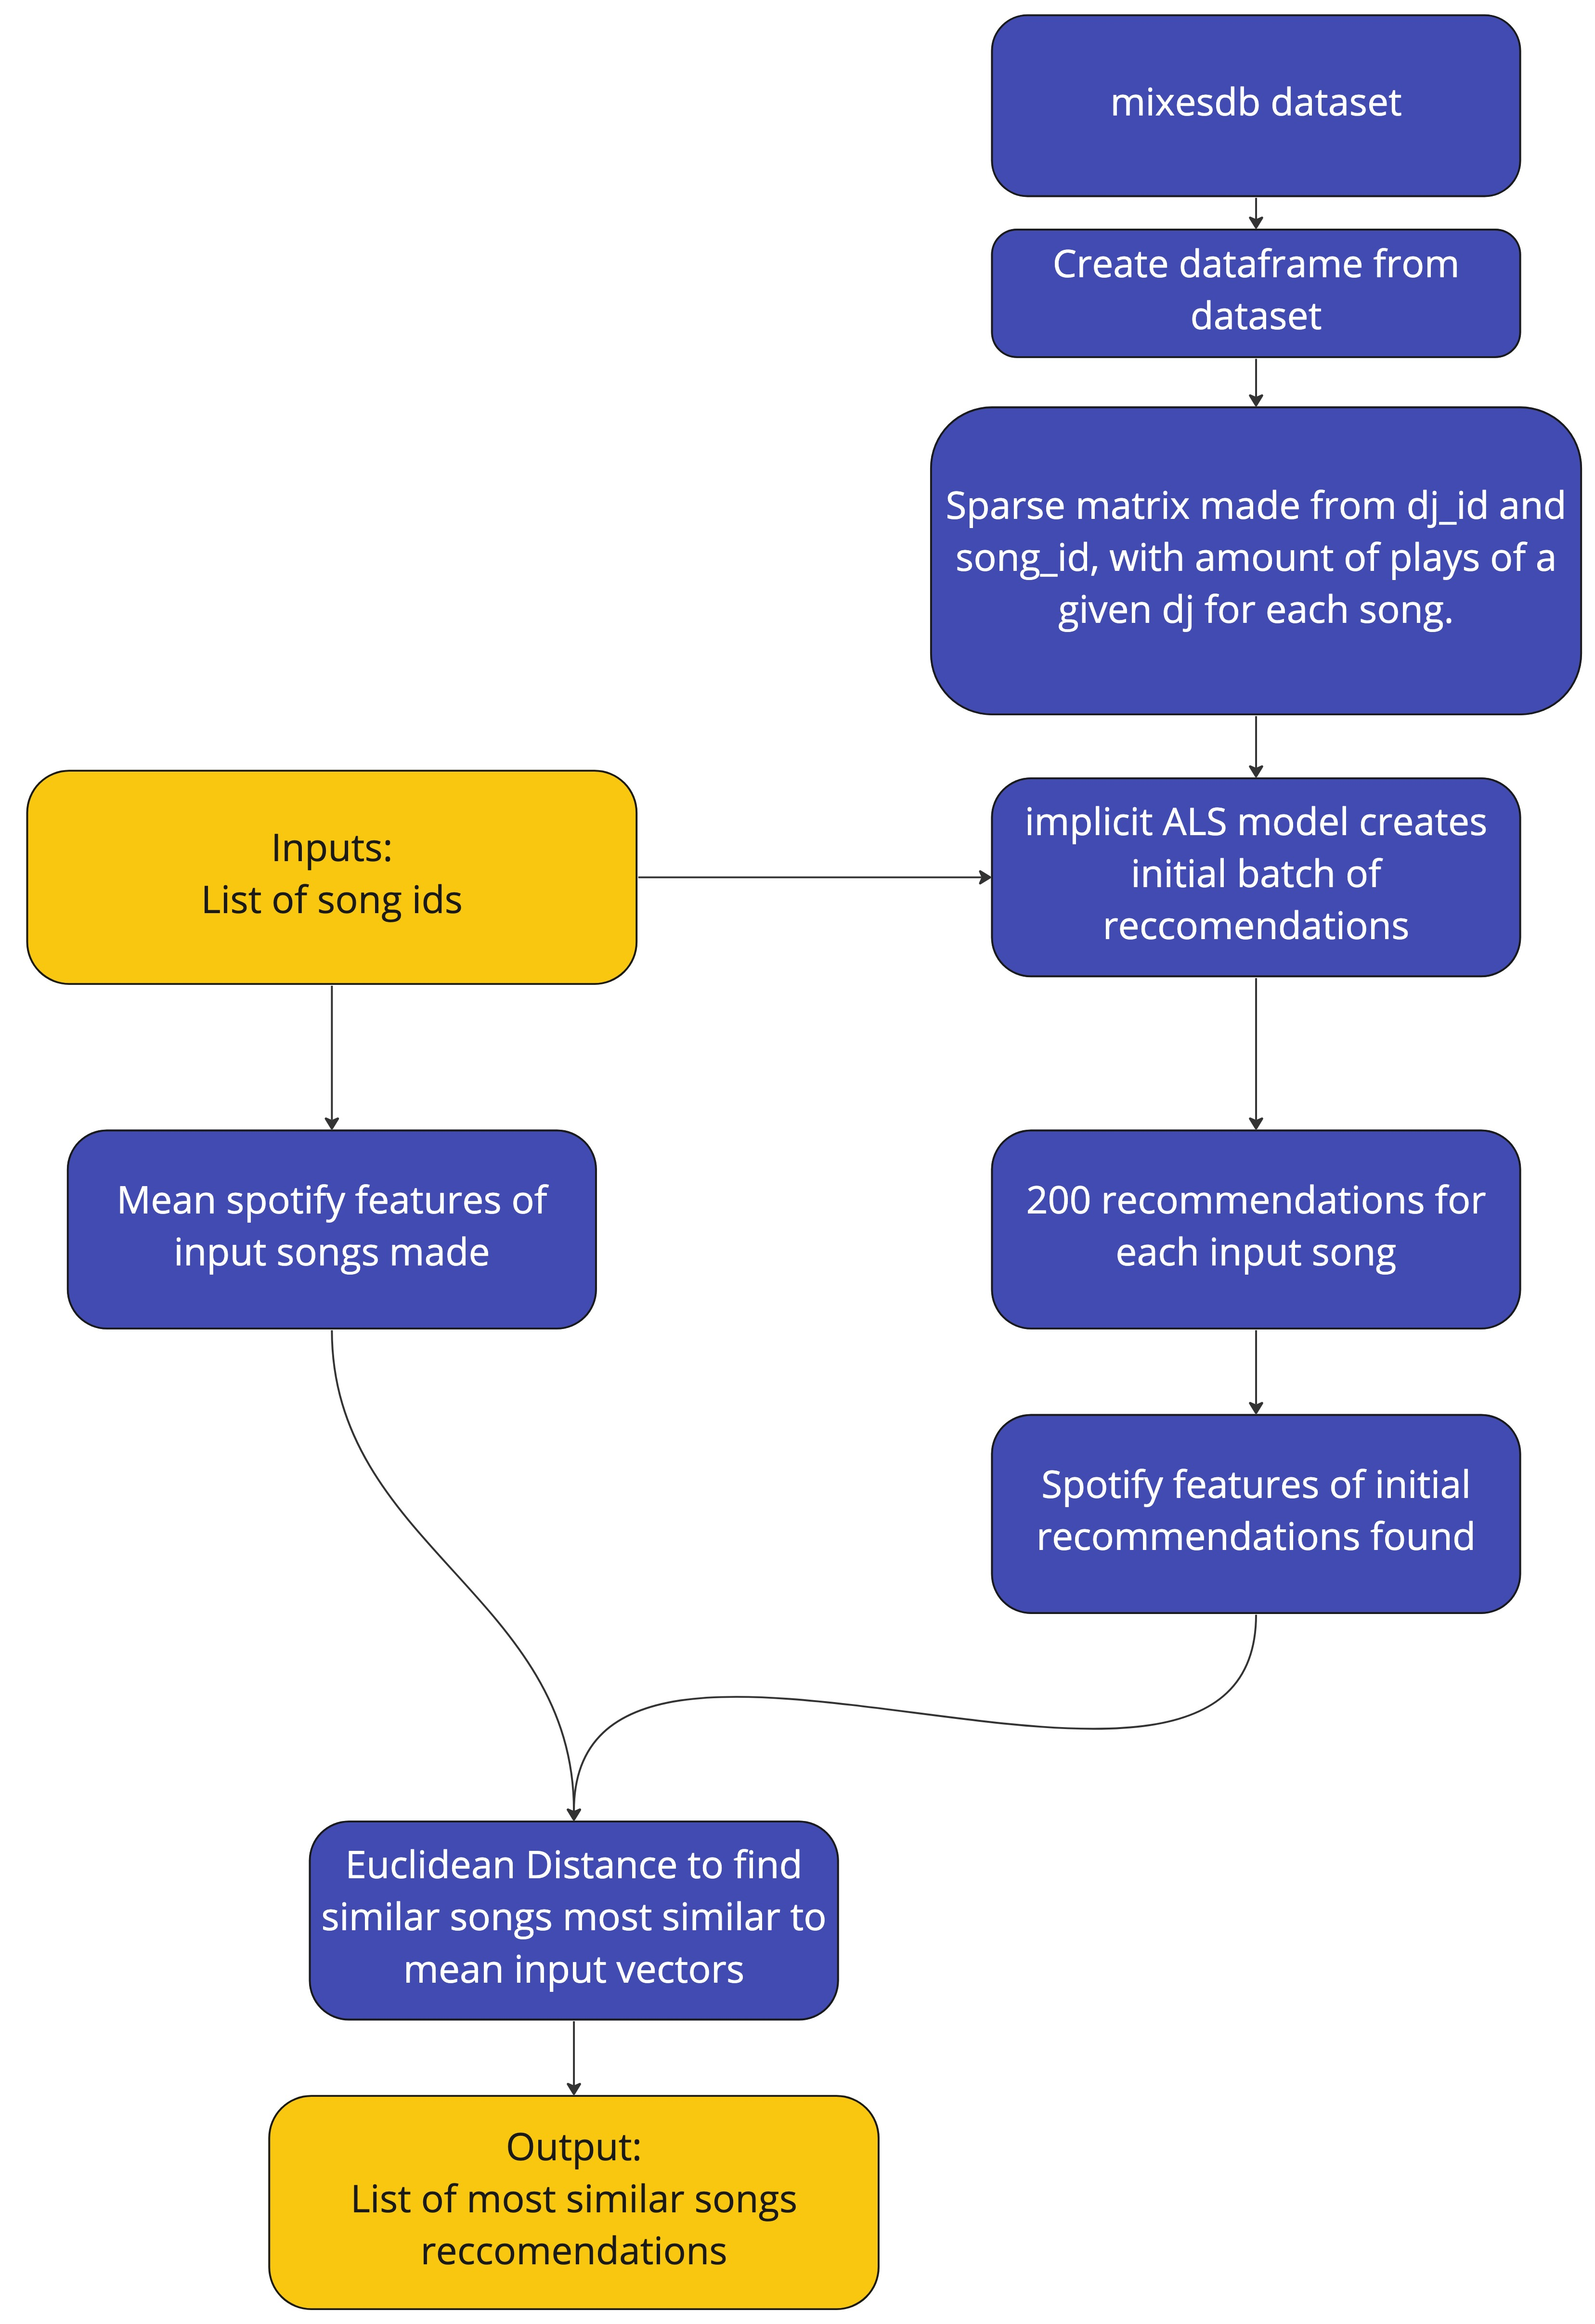
\includegraphics[scale=0.1]{images/application_app_flow}
	\centering
	\caption{Application flow of the final suggestions part} 
\end{figure}

\subsection{Example Findings}
To demonstrate the application in a non methodical way. A variety of DJ Set tracklists corresponding to different genres were used as inputs for the application. and spotify playlists of these recommendations can be found below.  Three different DJ sets: were used.

\begin{center}
	\begin{tabular}{ |c|} 
		\hline
		Moxie, Shanti Celeste, Chris Farrell - NTS Radio\\ 
		\hline \textbf{Input Songs}\\ 
		\hline Escape Earth \textit{Gravity Well} \\ 
		\hline Priori \textit{6thematic }\\
		\hline Carter Bros. \textit{Run - Monty's Bonus Beats}\\
		\hline Tyler Dancer \textit{Karmán Line}\\ 
		\hline Anunaku \textit{Forgotton Tales}\\
		\hline Piezo \textit{Tinned}\\
		\hline KMA Production \textit{Cape Fear}\\
		\hline Parris \textit{Dusty Glass Bubbles}\\
		\hline Tornado Wallace \textit{Open Door - Born Inna Tent Mix}\\
		\hline Luke Slater \textit{I Want You Too}\\
		\hline \textbf{Recommended Songs}\\ 
		\hline Black Booby \textit{Fill My Cup}\\
		\hline Omar S, John FM \textit{Heard'chew Single}\\
		\hline Hammer \textit{Manaka}\\
		\hline Awanto 3 \textit{Pregnant}\\
		\hline Steve Murphy \textit{Next Saturday - Club Mix}\\
		\hline Chasindub \textit{Still Here}\\
		\hline Ian Pooley \textit{Swing Mode}\\
		\hline Hashin \textit{Al-Naafyish (The Soul) - The "It's" About "Time" Remix}\\
		\hline Synkro \textit{Look at Yourself}\\
		\hline Awanto 3 \textit{Pregnant}\\
		\hline
	\end{tabular}
\end{center}

\begin{tabular}{ |p{3cm}|}
	\hline
	\multicolumn{1}{|c|}{Moxie, Shanti Celeste, Chris Farrell - NTS Radio:} \\
	\hline
	\textbf{Input Songs}\\
	\hline
	Escape Earth - Gravity Well \\
	Priori - 6thematic\\
	Albania \\
	Algeria \\
	American Samoa\\
	Andorra\\
	Angola\\
	\hline
\end{tabular}

\begin{itemize}
	\item \textbf{Rory Bowens, PLO Man, C3D-E, Brian Not Brian - The Slip, NTS Radio: } 
	\begin{itemize}
		\item \textbf{Genre:} New wave \& House
		\item \textbf{Tracks available:} 3/21
		\item \textbf{Input Link:} \hyperlink{sdsd}{https://open.spotify.com/playlist/0i4DAcdhMWRwNui9dHnb1i?si=7acf6675d5c448cf}
		\item \textbf{Output Link:} 3/21
	\end{itemize}
	\item \textbf{Moxie, Shanti Celeste, Chris Farrell - NTS Radio: } 
	\begin{itemize}
		\item \textbf{Genre:} Tech-House
		\item \textbf{Tracks available:} 10/28
		\item \textbf{Input Link:} 3/21
		\item \textbf{Output Link:} 3/21
	\end{itemize}
	\item \textbf{Chimpo b2b L U C Y @ Keep Hush Live: Sherelle Presents:}
	\begin{itemize}
		\item \textbf{Genre:} Jungle \& Breaks
		\item \textbf{Tracks available:} 8/
		\item \textbf{Input Link:} 3/21
		\item \textbf{Output Link:} 3/21
	\end{itemize}
	
\end{itemize}

When going through the recommended songs, the BPMs of the output songs were observed to see if they were around the same range as the input songs. The songs were listened to see if stylistically they were similar to the input songs, and the source of the recommended songs were also observed.

The Slip set performed okay. Expectations were low due to the small amount of tracks available. Two of them had a House style to them and one was Indie. The output songs were all house songs and none matched stylistically to the one indie song. However, all the BPM's were in a similar range around 110-120 BPM. The Moxie set performed very well. The input songs were all Tech-House songs which had a bit of a strange vibe and the output songs were that as well as some more disco centric tunes. BPM's were all very similar as well. The Keep Hush set also performed well. The BPM ranges were similar to the input songs and stylistically matched the input songs well. All the suggested tunes did not come from an eclectic mix of DJ Sets or DJs, in each batch of suggestions youd see songs either from the same mix or the same DJ. This is most likely due to the sparsity of the dataset. Links to each input and recommended DJ set can be found in the appendix.

The intent of displaying this is more to show the application in action rather than dissecting the quality of its performance which is analysed in the Experiment chapter.

